\documentclass[12pt,a4paper]{article} 

\usepackage{amsmath,amsfonts,amssymb,latexsym,graphicx,array}
\usepackage[french]{babel}
\usepackage[T1]{fontenc} 
\usepackage[utf8]{inputenc}
\usepackage{color}
\usepackage[a4paper, margin={3cm, 3cm}]{geometry}
\usepackage{subfigure}
\usepackage{epstopdf}



\begin{document}
%%%%%%%%%%%%%%%%%%%%%%%%%%%%%%%%%%%%%%%%%%%%%%%%%%%%%%%%%%%%%%%%%%%%%%%%%%%%%%%%%%%%%%%%%%%%%
% page titre
%%%%%%%%%%%%%%%%%%%%%%%%%%%%%%%%%%%%%%%%%%%%%%%%%%%%%%%%%%%%%%%%%%%%%%%%%%%%%%%%%%%%%%%%%%%%%
\setcounter{page}{0}


\begin{center}

% logo
\begin{minipage}[l]{.49\linewidth}
	\flushleft
\includegraphics[width=4cm]{img/logo_ENSTA.jpg}
\end{minipage}
\begin{minipage}[r]{.49\linewidth}
	\flushright
\includegraphics[width=4cm]{img/logo_CNAM.png}
\end{minipage}
\vspace{1.5cm}

% titre
\hrule \vspace{0.5cm}
\begin{LARGE}
	\textbf{FAT -- Projet Vélib}\\
\end{LARGE}
\vspace{0.5cm} \hrule
\vspace{3cm}

% noms
\definecolor{carmine}{rgb}{0.59, 0.0, 0.09}
\begin{Large}\color{carmine}
	Emmanuel JAY\\
	Adrien MAR\'ECHAL\\
	Benoît MULOCHER\\
\end{Large}
\vspace{5cm}

% Nom écoles
\begin{large}
	\textit{Conservatoire National des Arts et Métiers\\
	--\\
	\'Ecole Nationale Supérieure de Techniques Avancées\\}
\end{large}
\vfill

% date
\today
\end{center}

\thispagestyle{empty}
\newpage

%%%%%%%%%%%%%%%%%%%%%%%%%%%%%%%%%%%%%%%%%%%%%%%%%%%%%%%%%%%%%%%%%%%%%%%%%%%%%%%%%%%%%%%%%%%%%
%%%%%%%%%%%%%%%%%%%%%%%%%%%%%%%%%%%%%%%%%%%%%%%%%%%%%%%%%%%%%%%%%%%%%%%%%%%%%%%%%%%%%%%%%%%%%


\section{Définition du modèle}

\begin{figure}[h]
	\centering
	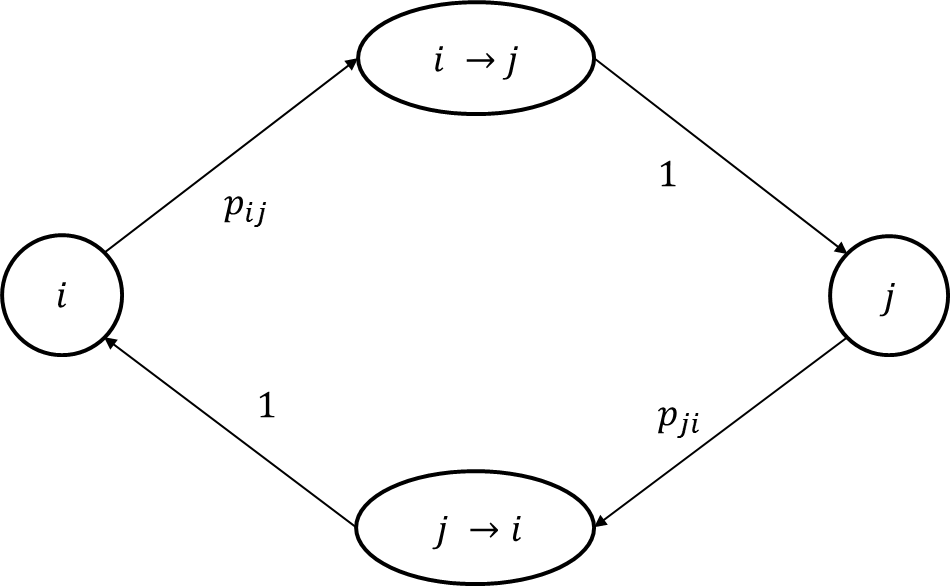
\includegraphics[width=0.6\linewidth]{img/modele.png}
	\caption{Schéma succinct du modèle de base, où uniquement 2 nœuds/stations et les trajets les reliant sont représentés. Les valeurs sur les arcs indiquent les probabilités de transition.}
	\label{fig:1}
\end{figure}

On intègre à notre modèle à la fois une représentation des stations vélib, et également des tous les trajets possibles entre ces stations. On a ainsi des nœuds $i$ qui correspondent aux stations et des nœuds $i\rightarrow j$, notés $(ij)$, qui correspondent au trajets entre les stations, $i$ et $j$ décrivant l'ensemble des stations, qui sera noté assez explicitement $stations$ et sera parfois assimilé à l'ensemble $[\![1,n]\!]$ en numérotant arbitrairement les stations.

Les nœuds sont ici en fait des \textit{colonies} telle qu'elles sont décrites dans le chapitre 2.3 du livre de Kelly (ajouter ref). On reprendra dans toute la suite les notations développées par Kelly.\\


On note dès lors $T_{a,b}(n)$ l'opérateur de transition, avec $(a,b) \in \left\{ \left(i,(ij)\right), i,j \in stations \right\} \cup \left\{ \left((ij),j\right), i,j \in stations \right\}$.
\[
T_{a,b}(n) = (...,n_a - 1,..., n_b + 1, ...)
\]

Les taux de transition sont écrits
\[
q\left(n, T_{a,b} (n) \right) = \lambda_{a,b} \phi_b(n_b)
\]
avec $\lambda_{a,b} = (proba\_transition\_a\_b) \times (temps\_service\_en\_a)$\\

On note $\lambda_a = \sum_b \lambda_{a,b}$ le paramètre du temps de service en $a$.
Lorsque $a = i$ est une stations, $\lambda_i$ correspond au taux de départ (horaire) de la station. Lorsque l'on considère un trajet $a = (ij)$, $\lambda_{(ij)}$ correspond au temps de trajet entre $i$ et $j$.\\


En notant $p_{ij}$ la probabilité d'emprunter le chemin vers $j$ depuis la stations $i$ (i.e. la proba de la transition $\left(i,(ij) \right)$), on a
\begin{equation}
\lambda_{i,(ij)} = p_{ij} \lambda_i
\end{equation}

D'autre part, comme on a des probabilités de transition égales à $1$ depuis un chemin vers sa destination, on a
\begin{equation}
\lambda_{(ij),j} = \lambda_{(ij)}
\end{equation}


\section{Matrice de routage}

Pour trouver la matrice de routage à partir des données, nous avons décidé d'utiliser l'artillerie lourde. Nous avons utilisé l'interface python de Cplex pour faire un script, qui, à partir des données, résoud un programme quadratique dont les variables sont les coefficients de la matrice de routage.
On choisis de minimiser la somme des carrés des coefficients, afin que le résultat obtenu soit le plus équilibré possible (que depuis chaque station, on aille de façon équitable aux autres stations en fonction des contraintes)
\[ 
	\min \sum_{i,j} p_{i,j}^2
\]
Sous les contraintes de probabilité :
\[
	\sum_{j=1}^n p_{i,j} = 1 \qquad \forall i \in [\![1,n]\!]
\]
De cohérence avec les données
\[
	\sum_{i=1}^n departure[i]*p_{i,j} = arrival[j] \qquad \forall j \in [\![1,n]\!]
\]
Et du fait qu'on ne puisse pas revenir a une station
\[
	p_{i,i} = 1 \qquad \forall i \in [\![1,n]\!]
\]


\section{\'Equations de trafic}

L'équation de trafic $(2.1)$ du livre de Kelly, après avoir fait apparaître les probabilités de transition, devient pour notre problème, avec $(\alpha_a), a \in \left\{ i \in stations \right\} \cup \left\{ (ij), i,j \in stations \right\}$  la distribution à l'équilibre :
\begin{equation}
\alpha_{(ij)} \lambda_{(ij)} = \alpha_i p_{ij} \lambda_i
\label{eq:trafic_1}
\end{equation}
pour une transition à travers un chemin $(ij)$, et
\begin{equation}
\alpha_j \sum_k p_{jk} \lambda_j = \sum_k \alpha_{(kj)} \lambda_{(kj)}
\label{eq:trafic_2}
\end{equation}
pour une transition par une station $j$.

Comme $\sum_k p_{jk} = 1$, on a donc
\begin{equation}
\alpha_j \lambda_j = \sum_k \alpha_{(kj)} \lambda_{(kj)}
\label{eq:trafic_2_bis}
\end{equation}
pour la transition par la station $j$.\\

En injectant l'expression des $\alpha_{(ij)}$, on obtient
\begin{equation}
\alpha_j = \frac{1}{\lambda_j} \sum_i \alpha_i p_{ij} \lambda_i
\label{eq:trafic_2_ter}
\end{equation}


Par ailleurs, on a les conditions
\[
\alpha_i > 0, \quad \alpha_{(ij)} >0, \quad \forall i,j \in stations 
\]
et
\begin{equation}
\sum_i \alpha_i + \sum_i \sum_j \alpha_{(ij)} = 1
\end{equation}
i.e.
\begin{equation}
\sum_i \left(1 + \lambda_i \sum_j \frac{p_{ij}}{\lambda_{(ij)}} \right) \alpha_i = 1
\label{eq:contrainte}
\end{equation}

~\\
Pour résoudre ces \textit{équations de trafic}, on réécrit l'équation (\ref{eq:trafic_2_ter}) sous forme matricielle
\begin{equation}
\alpha = \alpha P
\end{equation}
où $\alpha$ est le vecteur ligne des $\alpha_i, i \in stations$. Et $P$ est la matrice dont les coefficients sont donnés par $\left( p_{ij} \frac{\lambda_i}{\lambda_j} \right)_{i,j \in stations}$.\\

La résolution de ce système doit ensuite être menée en tenant compte de la contrainte (\ref{eq:contrainte}). Pour ce faire, il suffit d'inverser la matrice $(I-P)$ dans laquelle on a remplacé une colonne par le vecteur formés par $\left(1 + \lambda_i \sum_j \frac{p_{ij}}{\lambda_{(ij)}} \right)_{i \in stations}$, et on utilisant un second membre nul, sauf pour la colonne correspondant à celle modifiée qui doit comporter un $1$.
 
On calculera ainsi les $\alpha_i$, d'où découlerons ensuite les $\alpha_{(ij)}$ (si tant est qu'ils nous intéressent) grâce à l'équation (\ref{eq:trafic_1}).\\

Les solutions des équations de trafic nous permettent ensuite de calculer la distribution stationnaire d'un processus migratoire basé sur notre modèle (en accord avec le théorème 2.4 du livre de Kelly).



\section{Modèle du Système}

Nous ponvons donc modéliser notre problème de stations avec les coefficients suivants, pour $i,j$ des stations différentes et $ij$ représentant le chemin entre $i$ et $j$:

\paragraph*{}
Coefficients du générateur infinitésimal pour une transition entre une station, et un chemin de cette station vers une autre:
$$
q(n, T_{i,ij} (n)) = p_{i,j} * min(1,n_i)
$$

\paragraph*{}
Coefficients du générateur infinitésimal pour une transition entre un chemin et la station d'arrivée :
$$
q(n, T_{ij,j} (n)) = \mu_{i,j} * n_{ij} \;\;\; if(n_j != n^{max}_j)
$$
$$
q(n, T_{ij,j} (n)) = 0 \;\;\; if(n_j == n^{max}_j)
$$

\paragraph*{}
Le reste des coefficients du générateur infinitésimal est nul


\end{document}